
In this section we develop the Capsule model.  Capsule captures patterns in entity behavior and identifies events that cause deviations from these patterns among many entities.  The model relies on rich entity behavior data over time, such as messages being sent between entities; text data can summarized (making the model more tractable) with a topic model~\cite{Blei:2012}.  We first review topic models at a high level and give the intuition on Capsule.  Then, we formally specify our model and discuss how we learn the hidden variables.

\parhead{Background: Topic Models.} Capsule relies on topic models to summarize text data, making the model tractable.  Topic models are algorithms for discovering the main themes in a large collection of documents; each document can then be summarized in terms of the global themes.  More formally, a topic $k$ is a probability distribution over the set of vocabulary words.  Each document $d$ is represented as a distribution over topics $\theta_d$.  Thus we can imagine that when we generate a document, we first pick which topics are relevant (and in what proportions); then, for each word, we select a single topic from this distribution over topics, and finally select a vocabulary term from the corresponding topic's distribution over the vocabulary.  We use the LDA topic model~\cite{Blei:2003,Hoffman:2010} to summarize text data, and assume that these summaries are held fixed.  Our model could be extended to include topic modeling as component, but in practice the results would be similar to the stage-wise approach.

\parhead{The Capsule Model.}
Topic models are often applied to provide a structure for an otherwise unstructured collection of documents.  Documents, however, are often accompanied by metadata, such as the date written or author attribution; this information is not exploited by traditional topic models.  The Capsule model uses both author and date information to identify and characterize events that influence the content of the collection.

Consider an entity like the Bangkok American embassy, shown in Figure~\ref{fig:cartoon}.  We can imagine that there is a stream of messages (or \emph{diplomatic cables}) being sent by this embassy---some might be sent to the US State Department, others to another American embassy like Hong Kong.  An entity will usually talk about certain topics; the Bangkok embassy, for instance, is concerned with topics regarding southeast Asia more generally.

Now imagine that at a particular time, an event occurs, such as the capture of Saigon during the Vietnam war.  We do not directly observe that events occur, but each event can again be described in the same topic space used to describe individual messages.  Further, when an event occurs, the message content changes for multiple entities. The day following the capture of Saigon, the majority of the diplomatic cables sent by the Bangkok embassy were about Vietnam war refugees.
Thus we imagine that an entity's stream of messages is controlled by what it usually talks about as well as the higher level stream of unobserved events.

\parhead{Model Specification.}
% We formally describe Capsule. The observed data are documents represented in topic space; each document has an author (or entity) and a time (or date) associated with it.  The document content for each document $d$ is represented as $\theta_d$, a $K$-dimensional vector, where $K$ is the number of topics.  The author and time associated with document $d$ are represented as $n_d$ and $m_d$, respectively.

% The hidden variables of this model are the authors' typical concerns, event occurrences, and event descriptions.  We represent the concerns of author $n$ as $\phi_n$, also a $K$-dimensional topic vector.  For each time $t$ we represent whether or not an event occurs with $\epsilon_t$; when an event does occur we represent its content as $\pi_t$, another $K$-dimensional topic vector.

% Conditional on the hidden variables and the author and time metadata, Capsule is a model of how document topics $\theta_d$ came to be; we generate the topics for each document
% \begin{equation}
% \theta_{d,k} \sim \mbox{Gamma}\left(\phi_{n_d,k} + \sum_{t=1}^T f(t, m_d) \epsilon_t \pi_{t,k}\right),\footnotemark
% \end{equation}
% % \footnotetext{Throughout this work, we use a non-traditional parameterization of the gamma distribution.  Recall the shape $a$ and scale $b$ parameterization of the gamma, or \[\mbox{Gamma}^*(x \g a, b) = \frac{1}{\Gamma(a) b^a} x^{(a-1)}e^{- x / b}.\] In our alternative parameterization, we use a single mean parameter $\mu$ and a fixed sparsity hyperparameter $\alpha$, or \[\mbox{Gamma}(x \g \mu, \alpha) = \mbox{Gamma}^*(x \g \alpha, \mu / \alpha);\] when a gamma distribution is only specified by a single parameter, it is the mean $\mu$ and the sparsity hyperparamter $\alpha$ is hidden for simplicity.
% % }
% where we define the event decay function $f$ to be a simple linear decrease: \[f(t, m) =
% \begin{cases}
%   1 - \frac{m-t}{\delta}, & \mbox{if } t \le m < t+\delta \\
%   0, & \mbox{otherwise,}
% \end{cases} \] with $\delta$ being the time duration after the event at time $t$ is no longer relevant.  Figure~\ref{fig:graphicalmodel} shows the dependencies between the hidden and observed variables as a graphical model.

% To complete the specification of all the variables, we place priors on all of the hidden variables.  Author concerns $\phi_{n,k}$ and event content $\pi_t$ are specified with Gamma priors.  Event occurrence $\epsilon_t$ has a Poisson prior.
% % TODO: we make a note about the Poisson taking values > 1; what is the intuition?

% \begin{figure}
% \centering
% 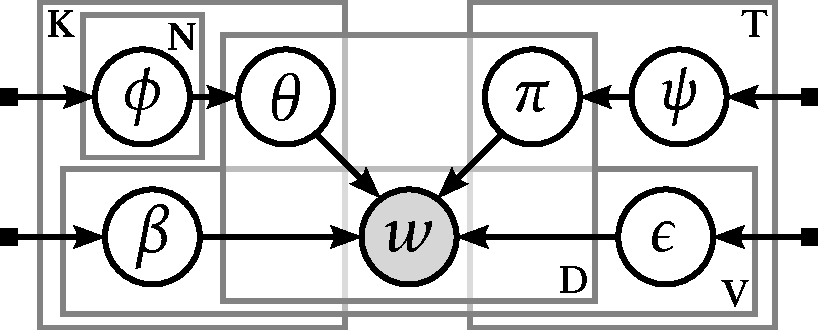
\includegraphics[width=0.5\linewidth]{fig/graphicalmodel.pdf}
% \caption{A directed graphical model of Capsule to show considered dependencies. Shaded document topics nodes $\theta$ are observed. unshaded nodes are hidden variables---these are event occurrences $\epsilon$, event content descriptions $\pi$, and entity typical concerns $\phi$. Plates denote replication: there are $D$ documents, $T$ time steps, $N$ entities, and $K$ topics. Hyperparameters $\eta$, $\mu$, and $\alpha$ are fixed.}
% \label{fig:graphicalmodel}
% \end{figure}

Option 1:
\begin{itemize}
\item for each topic $k \in \{1,\dots, K\}$:
	\begin{itemize}
	\item draw topic distribution over vocabulary $\beta_k \sim \mbox{Dirichlet}_V (\alpha)$
	\item for each entity $n \in \{1,\dots, N\}$:
		\begin{itemize}
		\item draw entity concerns $\phi_{n,k} \sim \mbox{Gamma}(s_\phi, r_\phi)$
		\end{itemize}
	\end{itemize}
\item for each time step $t \in \{1,\dots, T\}$:
	\begin{itemize}
	\item draw event description over vocabulary $\pi_t \sim \mbox{Dirichlet}_V (\alpha)$
	\item draw event strength $\psi_{t} \sim \mbox{Gamma}(s_\psi, r_\psi)$
	\end{itemize}
\item for each document $d$ with author $a_d$ at time $i_d$:
	\begin{itemize}
	\item draw local entity concerns $\theta_{d,k} \sim \mbox{Gamma}(s_\theta, \phi_{a_d,k})$ (for each topic $k \in \{1,\dots, K\}$)
	\item draw local event strength $\epsilon_{d,t} \sim \mbox{Gamma}(s_\epsilon, \psi_{i_d,t})$ (for each time $t \in \{1,\dots, T\}$)
	\item draw $w_{d,v} \sim \mbox{Poisson}(\theta_d^\top\beta_v + \sum_{t=1}^T f(i_d, t) \epsilon_{d,t} \pi_{t,v} )$ (for each vocabulary term $v \in \{1,\dots,V\}$)
	\end{itemize}
\end{itemize}

+ easier to describe sampling from D documents for inference
+ graphical model will be more intuitive / cleaner
+ easier to tell what parameters are local (document level) or global
- we need to explicitly state how to map document d to its corresponding author and time



Option 2:
\begin{itemize}
\item for each topic $k \in \{1,\dots, K\}$:
	\begin{itemize}
	\item draw topic distribution over vocabulary $\beta_k \sim \mbox{Dirichlet}_V (\alpha)$
	\item for each entity $n \in \{1,\dots, N\}$:
		\begin{itemize}
		\item draw entity concerns $\phi_{n,k} \sim \mbox{Gamma}(s_\phi, r_\phi)$
		\end{itemize}
	\end{itemize}
\item for each time step $t \in \{1,\dots, T\}$:
	\begin{itemize}
	\item draw event description over vocabulary $\pi_t \sim \mbox{Dirichlet}_V (\alpha)$
	\item draw event strength $\psi_{t} \sim \mbox{Gamma}(s_\psi, r_\psi)$
	\end{itemize}
\item for each sender/author $i$, recipient $j$ at time $d$:
	\begin{itemize}
	\item draw local entity concerns $\theta_{i,j,d,k} \sim \mbox{Gamma}(s_\theta, \phi_{i,k})$ (for each topic $k \in \{1,\dots, K\}$)
	\item draw local event strength $\epsilon_{i,j,d,t} \sim \mbox{Gamma}(s_\epsilon, \psi_{d,t})$ (for each time $t \in \{1,\dots, T\}$)
	\item draw $w_{i,j,d,v} \sim \mbox{Poisson}(\theta_{i,j,d}^\top\beta_v + \sum_{t=1}^T f(d, t) \epsilon_{i,j,d,t} \pi_{t,v} )$ (for each vocabulary term $v \in \{1,\dots,V\}$)
	\end{itemize}
\end{itemize}


+ it's very clear which authors correspond to what documents
- the receiver of the message doesn't play into the model, so why are we using it as an index? (corollary: makes it harder to argue that we can apply the model to arxiv abstracts)
- have to explain what happens if there are multiple documents at the same index (we add yet other index)
- visually, a variable with four indices is a little intimidating


\parhead{Learning the hidden variables.}
In order to use the Capsule model to explore the observed documents, we must compute the posterior distribution.  Conditional on the observed document topics $\theta$, our goals to to compute the posterior values of the hidden parameters---event occurrences $\epsilon$ and descriptions $\pi$, as well as entity concerns $\phi$.

As is common for Bayesian models, the exact posterior for Capsule is not tractable to compute; approximating it is our central statistical and computational problem.  We develop an approximate inference algorithm for Capsule based on variational methods~\cite{Wainwright:2008}.\footnote{Source code available at https://github.com/ajbc/capsule.\\ TODO: release on github repo (this link is not active.)  submission is not anonymous, so why not?}

Variational inference approaches the problem of posterior inference by minimizing the KL divergence from an approximating distribution $q$ to the true posterior $p$.
This is equivalent to maximizing the ELBO: 
\begin{equation}
\mathcal{L}(q)  = \E_{q(\epsilon, \pi, \phi)}[\log p(\theta,\epsilon,\pi,\phi) - \log q(\epsilon, \pi, \phi)].
\label{eq:elbo}
\end{equation}

We define the approximating distribution $q$ using the mean field assumption:
\begin{equation}
q(\epsilon, \pi, \phi) = \prod_{t=1}^T q(\epsilon_{t} \g \lambda^\epsilon_t)\prod_{k=1}^K\left[\prod_{n=1}^N q(\phi_{n,k} \g \lambda^\phi_{n,k})\prod_{t=1}^T q(\pi_{t,k} \g \lambda^\pi_{t,k})\right].
\label{eq:q}
\end{equation}
The variational distributions $q(\pi)$ and $q(\phi)$ are both gamma-distributed with free variational parameters $\lambda^\pi$ and $\lambda^\phi$, respectively. The variational distribution $q(\epsilon)$ is Poisson-distributed with variational parameter $\lambda^\epsilon$.

The expectations under $q$, which are needed to maximize the ELBO, do not have a simple analytic form, so we use ``black box'' variational inference techniques~\cite{Ranganath:2014}.  Black box techniques optimize the ELBO directly with stochastic optimization~\cite{Robbins:1951}.  Full details on our inference algorithm can be found in the appendix.  This algorithm produces a fitted variational distribution which can then be used as a proxy for the true posterior, allowing us to explore a collection of documents with Capsule.  

\parhead{Visualization.}
Capsule is a high-level statistical tool. In order to understand and explore its results, a user must scrutinize numerical distributions.
To make Capsule more accessible, we developed an open source tool for visualizing its results.\footnote{Source code: https://github.com/ajbc/capsule-viz. TODO}  Our tool creates a navigator of the documents and latent parameters, allowing users to explore events, entities, topics, and the original documents.  Figure~\ref{fig:viz} shows several screenshots of this browsing interface.

\begin{figure}
\centering
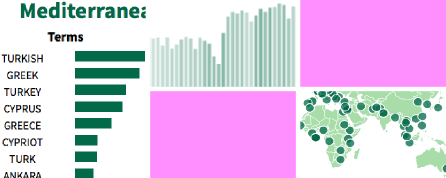
\includegraphics[width=\linewidth]{fig/viz.png}
\caption{Screenshots of Capsule visualization of US State Department cables.  Left: top words in a topic (manually labeled topic title).  Center-top: events over time (height is volume of messages sent, color is probability of an event occurring).  Center-bottom: topics for an event on <date TODO: cyprus coup?>.  Right-top: cyprus entity topics? TODO.  Right-bottom: entities shown on a map.}
\label{fig:viz}
\end{figure}
